\chapter{Introduction}
\index{Introduction@\emph{Introduction}}%

%\section{blah}
%\index{blah@\emph{blah}}%
%
%\texttt{asdf}
%
%\begin{quote}
%\index{guarantee}%
%This template package is provided and licensed ``as is'' without warranty
%of any kind, either expressed or implied, including, but not limited to,
%the implied warranties of merchantability and fitness for a particular
%purpose. Yadda, yadda, yadda, \ldots
%\end{quote}

This report presents a case study of applying W3C Web Components 
\index{Web Components}
to achieve encapsulation and separation of concerns within the context of collaborative web authoring. 
The author has created Speakur, a real-time discussion social plugin for the web, 
as an experiment to determine the maturity and viability of using Web Components to develop modern web applications.

Like most web apps, Speakur is primarily based on HTML and Javascript. 
The Hypertext Markup Language (HTML) 
\index{HTML}
document standard has proven wildly successful since its introduction in 1993 by British computer scientist 
Tim Berners-Lee, 
\index{Tim Berners-Lee}
with billions and billions of pages served, 
and millions of public and private web sites forming a major part of our information landscape. [CITE?]
More than any other invention other than perhaps email, the World Wide Web has shaped how we see and use the global network.

% 
\begin{figure}[htb]
\begin{center}
\ 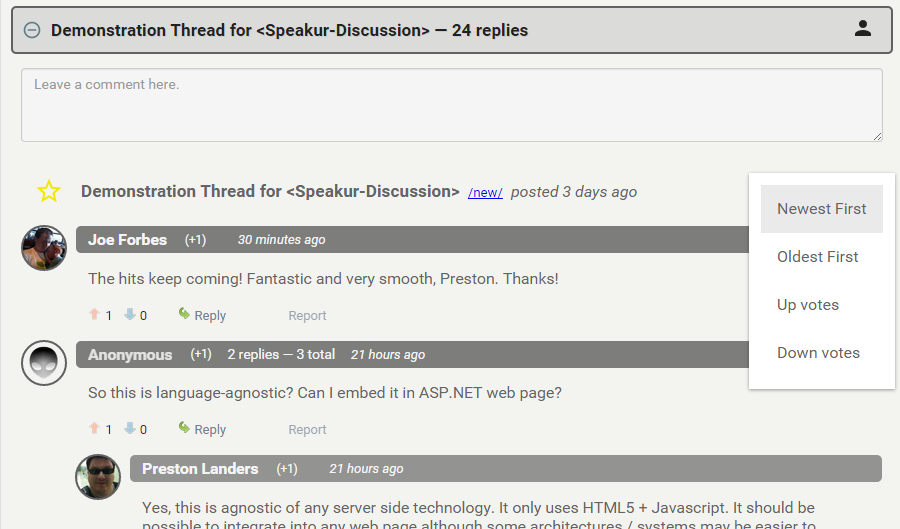
\includegraphics[width=6in]{images/screenshot_20150312_1630_v2.png}
\caption{A Speakur thread inside a demonstration page.}
\label{f:ex}
\end{center}
\end{figure}
\index{commands!environments!figure}%

Those designing and programming applications for the Web platform have long dreamed of the ability to mix and match independent, reusable chunks of functionality (components) in their documents without mutual interference. 
The original and current Document Object Model (DOM)
\index{DOM}
browser abstraction provided by HTML does not allow for significant decoupling; 
everything lives together on one big page. Hacks like the 
\tcode{<iframe>} 
\index{iframe}
tag have allowed one to work around some of these restrictions, 
but usually in an elegant and limited way.

At the time of HTML's introduction, 
the concept of quickly and easily composing a static web page, 
much less a full-fledged dynamic application, 
out of Lego-like reusable building blocks seemed like a distant dream at best. 
The introduction to web browsers of the Javascript
\index{Javascript}
\footnote[1]{Javascript, also rendered as JavaScript or JS, 
has no significant relation to Sun's (now Oracle's) popular Java programming language;
the name is an unfortunate coincidence at best.}
(JS) programming language in 1995 allowed for a completely new dimension of dynamic behavior that did not exist before.
Eventually web apps like Google Docs rivaled traditional desktop applications in functionality.
Still, web apps had to be stitched together `by hand' in ways that carefully ensured that the different parts worked together in perfect harmony or else disaster frequently ensued. 
Each component or area of the system could not help but be tied to the others at some level as a result of the programming model imposed by the DOM and HTML.

Over the years, going along with and perhaps helping to drive the growth of the web, 
Javascript grew in importance and a great many frameworks and libraries sprang up around the JS ecosystem to help manage this complexity and to provide structure to client side web apps.
For many years individual JS frameworks seemed to be as ephemeral as teenage pop idols as the industry searched for the Next Big Thing that would make writing high quality web apps less of bug-ridden, messy chore. 
In recent years Google's Angular [CITE] 
\index{Angular}
has emerged as a dominant client framework, 
due in part to its perceived high quality [CITE] and the fact that it represents an common point for a fragmented industry to rally around.
Facebook's React 
\index{React}
JS library with its Virtual DOM is an up-and-comer focused on high performance that is more complementary in nature to Angular than a true challenger.

Yet despite the recent successes of web frameworks like Angular and React in capturing developer attention, 
and the emergence of the updated HTML5 standard in 2011, 
there still did not exist a clear picture of how web apps could achieve the encapsulated component model that had become prevalent in other areas of software engineering.
That is, until engineers from Google 
\index{Google}
and Mozilla \index{Mozilla} \footnote{Sponsor of the popular Firefox web browser, this organization grew out Netscape whose Navigator browser helped first popularize the web.}
and other organizations got together to draft a new standard called Web Components that will extend and enhance HTML5 in interesting ways that could have unforeseen effects.

\section{Web Component Overview}
At its most fundamental level, the Web Component standard consists of 4 core DOM technologies that, 
if accepted by the World Wide Web (W3C) 
\index{W3C}
Consortium and web browser vendors, 
will eventually become native features provided by browsers and available to all web pages without any additional JS frameworks. The core Web Component technologies are:
\begin{itemize}
\item
\textbf{Custom Elements}: extending HTML with new elements---custom HTML tags
\item
\textbf{Shadow DOM}: encapsulation for the internals of custom elements
\item
\textbf{Templates}: scaffolding for instantiating blocks of HTML from inert templates
\item
\textbf{Imports}: packaging for HTML components
\end{itemize}

This paper will explore related web standards initiatives that are frequently associated with Web Components 
but not formally grouped under them such as mutation observers,
\index{mutation observers}
model driven views, 
\index{model driven views}
and the CSS Flexible Boxes
\index{Flex box} 
and CSS Grid
\index{CSS Grid}
systems. 
Because these technologies are not yet formally accepted as a W3C standard and not yet widely implemented in commonly used mobile and desktop browsers, 
Speakur has been implemented with Google's experimental Polymer framework.
Polymer provides a Javascript `polyfill'
\index{polyfill}
library to implement many of the new Web Component features in currently available browsers. 
Eventually this platform polyfill should become unnecessary, in theory, as WC becomes widely adopted in browsers.

The potential componentization of the web is one of the most exciting developments in web engineering in years and follows the overall growth in software-as-a-service (SaaS) 
\index{SaaS}
and service oriented architectures 
\index{Service Oriented Architecture}
as a organizational and deployment concept. 
The conversion of dynamic web logic---not mere snippets of plain HTML---into bundles of reusable, extendable, composable components enables web developers to move to a higher level of abstraction than was previously possible.

The move towards a component-based Web will enable all sorts of interesting new composite services, mashups, and help broaden the potential pool of web developers. 
It will do this by allowing authors to publish easily reusable `widgets' that can be easily juggled around and combined in novel ways that previously required a highly integrated (and hugely expensive) development model or lots of tedious glue code.


\section{Structure of This Paper}
\index{Structure of This Paper@\emph{Structure of This Paper}}%

The goal of this paper is to demonstrate the application of software engineering design patterns embodied in the  W3C proposed Web Components standard such as encapsulation, composition, and
automatic synchronization of application state. 
This paper attempts to explain many of the goals and principles of the Web Components initiative and show how a number of different technologies taken together help raise the overall level of abstraction for web authors and developers.

The Background section of this report provides an introduction some of the architectural problems inherent in modern web authoring and how Web Components (WC) attempts to address them. 
It also provides some background on software engineering design patterns that are embodied in Web Components such as encapsulation, composition, and inheritance, as well as technologies such as WebSockets and NoSQL databases.
It describes some of the motivations behind the development of Speakur and some of the specific software engineering questions it addresses, such as the ability to provide a hassle-free way to host an embedded discussion forum inside an arbitrary web resource in a way that is fully encapsulated.

The Approach section details the specific structures and techniques used when constructing a Web Component, and describes the technology and software architecture choices that went into Speakur. 
It describes how Speakur uses Web Components to implement encapsulated functionality that is protected 

The Implementation section describes the application of Web Component principles to the specific task of providing a flexible and suitably generic discussion forum / commenting system. 
It describes the overall architecture, code flow, and synchronization process. 
An important topic in this section is security: how can we implement a largely client-based system while maintaining some kind of data integrity?

This is followed by an Analysis section which discusses some of the outcomes as compared to the original goals and also looks at the impact of the selection of Web Components, Polymer, Firebase and some of the other architectural choices. A few quantitative results are included, I hope.

Finally, the Conclusion section is just all kinds of awesome and wraps up the paper. 

\section{Source Code and Demonstration Resources}
\index{Source Code and Demonstration Resources@\emph{Source Code and Demonstration Resources}}%

The source code for Speakur consists of HTML and Javascript code located in two git version control repositories. The first repository is for the actual
\tcode{<speakur-discussion>}
% \texttt{$\textless$speakur-discussion\textgreater} 
HTML element that is available for use by web authors, and the second contains additional demonstrations, a standalone application and a management console.

The public documentation to help web authors use Speakur in their own sites can be found here:

\tcode{\url{https://github.com/Preston-Landers/speakur-discussion}}

Demonstrations of several web pages which show off embedded Speakur discussions are available at the following location:


\tcode{\url{https://preston-landers.github.io/speakur-discussion/components/speakur-discussion-dist/demo.html}}
